
\documentclass[11pt, letterpaper]{article}
%\usepackage{bookmark}
\usepackage[a4paper,margin=2cm]{geometry}
\usepackage[]{graphicx}
\usepackage{bm}
\usepackage[strings]{underscore}
\usepackage{apacite}
\setlength{\parindent}{0pt}
\graphicspath{ {./Images} }
\usepackage{wrapfig}
\usepackage[autostyle, english = american]{csquotes}
\usepackage[toc,page]{appendix}
\MakeOuterQuote{"}
\begin{document}
\begin{titlepage}
	\title{roller coaster tycoon 2}
	\author{Noah Alexiou}
	\date{\today}
	
	\maketitle
	\centering

	
\end{titlepage}


\newpage
\tableofcontents


\newpage


\section{Formulation}
\subsection{Assumptions}
\begin{itemize}
	\item The terminology "smooth" was used to describe the required transition between pieces of track. It is assumed that this implied that at intersections, segments would be at same position, and have the same gradient.
	\item The task sheet specified "The beginning and end sections... have been erected and are in a perfectly straight alignment". While this did clarify that the first, and end pieces of track were parallel, their slope was not specified, and therefore assumed to be 0.
\end{itemize}




\subsection{Observations}
\begin{itemize}

	\item 

		\begin{figure}[h]
		
		\begin{center}
		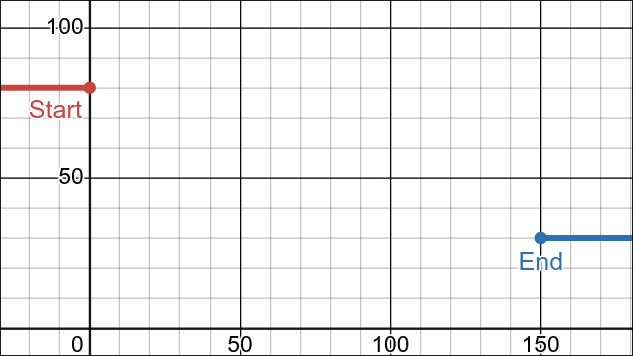
\includegraphics[width=15cm]{Start and End.png}

		\caption{The proposed start and end sections of the track}
		\end{center}


		\end{figure}

	\item The roller coaster was modelled in 2D to simplify calculations as graphing functions in 3D was out of the scope of the project. 
	\item The task sheet defined the success criteria as maximising exhilaration, caused by "swift changes in direction, height and steepness". 
		
	\item It was required that the track be constructed of at least 3 or more types of functions, including at least two types that are covered in Unit 3 Topic 2. The functions covered were exponential, logarithmic, and trigonometric functions.
	
	\item Trigonometric functions were calculated in radians, rather than degrees, in order for them to naturally oscillate more with smaller change in $x$.
	\item In order for the roller coaster to have sufficient speed to overcome any peaks or hills in the track, each successive peak should be at a lower height than any preceding it.

\end{itemize}



\subsection{Translation of aspects to Mathematical concepts and techniques}
\begin{itemize}
	\item Since the roller coaster had been assumed to be 2D, it's track was represented on the Cartesian plane. This allowed the use of desmos to graph its track and perform calculations by letting 1 unit be 1 meter. 
	\item The derivative function of modelled section of track could be used to determine the gradient at that point and therefore be used to determine if the track exceeded the specified "Maximum Slope for safety" requirement provided by the task sheet. In this case, it was $-2$.
	\item "Swift changes in direction, height and steepness" could be translated to swift changes in the $y-$axis, and gradient. However, there was a maximum gradient specified that must be considered. 
	\item In order to achieve as much of a thrill as possible, the maximum allowed slope should be reached whenever feasible.



\end{itemize}


\section{Solve}
\subsection{Modelling in Desmos}
\subsubsection{The First Function}
\begin{itemize}
	\item Considering that the starting point of the first function was 80 meters in the air, there was already sufficient height for the maximum gradient to be reached for a reasonable duration and  anticipation had already been built during the climb to the start.
	\item Clearly the first point will be $(80, 0)$ to connect with the start of the first segment. It was required that for the cubic function, say $f(x)=ax^3 +bx^2 +cx +d$, $f'(0)=0$. Since variables with $x$ coefficients 'drop out',$f(0)=0\Rightarrow c=0$.
	\item Since the derivative function was a quadratic, its lowest point could be considered the maximum slope reached by the original.
	\item The $x$-coordinates of the turning point of a quadratic could found using the vertex formula, which stated that for turning point $(x, y),\; x=\frac{-b}{2a}$.
	\item Considering the derivative function, $f'(x)=3ax^2+2bx$, it was found that the $x$-coordinates of the turning point were $\frac{-2b}{2\cdot3a}=\frac{-b}{3a}$.
	\item Therefore by finding $f'(\frac{-b}{3a})=-2$, a generic function could be found with minimum gradient -2, located at turning point. It was found that $f'(\frac{-b}{3a})=-2$ simplified to $b=\pm\sqrt{6a}$. Therefore the cubic $f(x)=ax^3\pm\sqrt{6a}x+d, a\geq0$ was found. 
	\item It was decided that the function inserted would be $f(x)=ax^3-\sqrt{6a}x+80, a\geq0$ as it placed the "drop" on the right hand side of the start of the coaster, and aligned the point on both tracks where their gradients were the same.
		\begin{figure}[h]
		\centering
		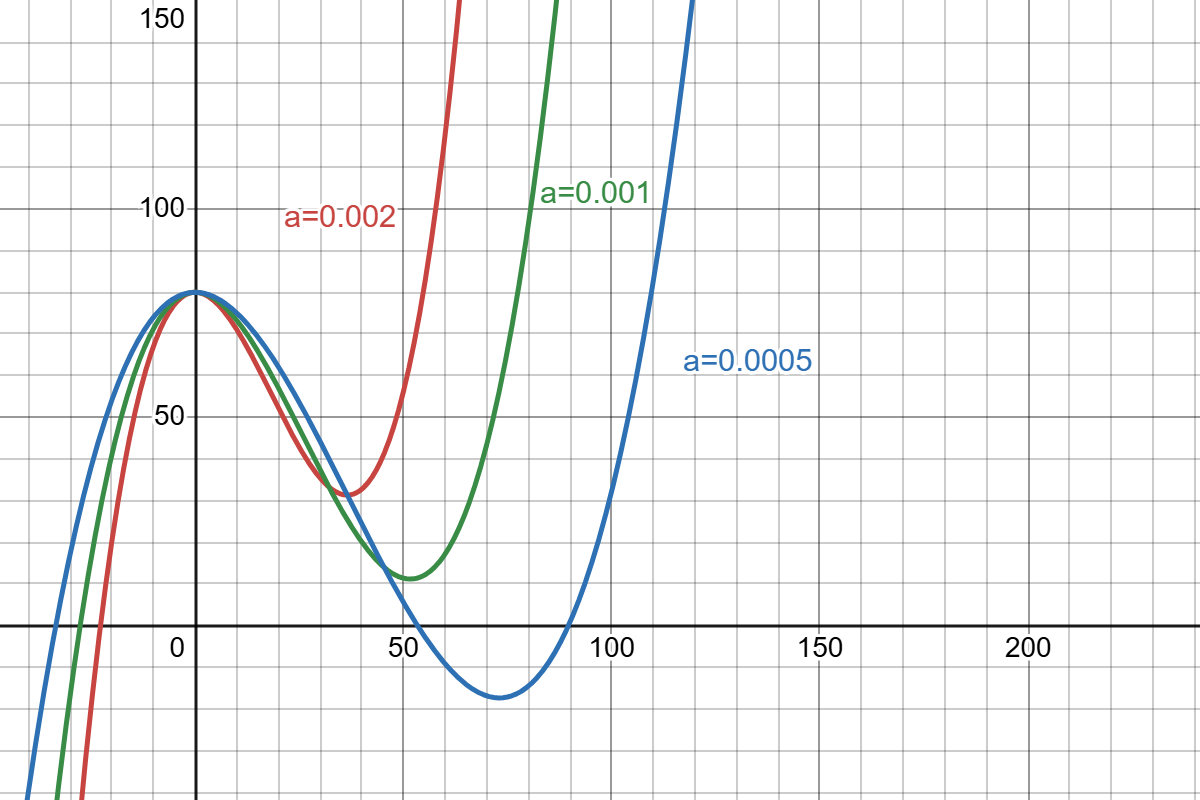
\includegraphics[width=15cm]{Eaxmple Cubic.png}
		\caption{Graphs of $f(x)=ax^{3}-\sqrt{6a}x^{2}+80$ with various $\mathbf{a}$ values}
	\end{figure}

	

	\item The end of the first function was chosen to be $f(30)$ as it was observed that letting it proceed further may have resulted in the end of the track being too low to the ground for a thrill to be achieved.
	\item It was required that the turning point be at $x=30$ so $f'(30)=0$ was considered. Solving for $a$ gave $a=\frac{2}{675}$
	\item Substituting this into $f(x)$ gave $f(x)=\frac{2}{675}x^{3}-\frac{2}{15}x^{2}+80$.
\end{itemize}
\subsubsection{The Second Function}
\begin{itemize}
	\item To connect the first and second functions, a point must be found where their gradients match.
	\item Consider $s(x)=a\sin(b(x+c))+d$. Therefore $s'(x)=ab\cos(b(x+c))$. Clearly the maximum downwards gradient was defined by $ab\cdot-1$, where $a,b \epsilon \mathbf{N}$, and $\cos(b(x+c))=-1$.
	\item However the peak of the next oscillation would be the same height than the previous one. Therefore if the function  had to be modified as to maintain sufficient speed to overcome the next peak. This was achieved though the creation of a new function, $c(x)=a\sin(b(x+c))+d+gx$, so that $c'(x)=ab\cos(b(x+c))+g$.
	\item Clearly now when $g<0$, the function will slope downwards throughout its oscillation. 

	\begin{figure}[h]
		\centering
		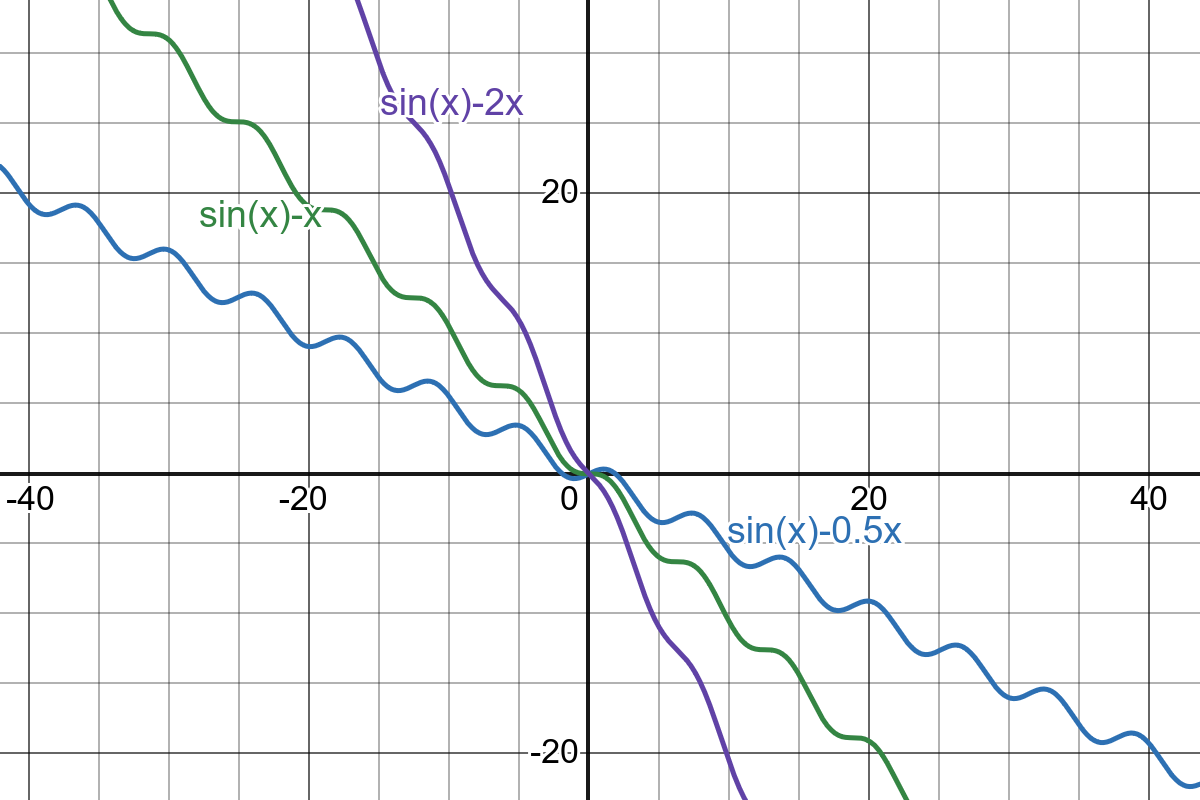
\includegraphics[width=15cm]{c(x).png}
		\caption{The function $y=sin(x)$ with various slopes applied}
	\end{figure}
	
	\item By letting $g=-0.1$, suitable values for $a$ and $b$ could be resolved. Clearly $ab\cdot -1-0.1=-2$ would result in a minimum gradient of $-2$. Therefore through trial and error in Desmos it was found that for $c'(x)=-2$, $a=9.5,b=0.2$ were appropriate. Therefore all that was left to do was to let $f'(x)=c'(x)$, shifting horizontally until the minimums were at the same $x$ co-ordinates, then shift vertically shift using $d$ until the functions met.  
	\item It was found  that $9.5\cdot0.2\cos (0.2(30+c))-0.1=0 \Rightarrow c=-6.174775557$, and therefore $9.5sin(0.2(30-6.174775557))+d+3=40 \Rightarrow d=52.48683298$
\end{itemize}
\subsubsection{The Third Function}
\begin{itemize}
	\item It was decided that the third function would be an exponential with an increasing downwards slope.
	\item Considering the general form of an exponential, $g(x)=ae^{b(x+c)}+d$, it was found that solving for variables $a, b, c$ and $d$ would require significant computation.
	\item Therefore it was decided that only $a$ and $b$ would need to be solved for, while $c=0$, and $d=0$.
	\item The point $(80, 0)$ was considered the origin for $g(x)$ during computation, so that  initial requirements such as $g(80)=c(80)$ became $g(0)=c(80)$. 
	\item Now that $g(x)=ae^{bx}$, $g'(x)=abe^{bx}$, we could solve for $a$ and $b$ using simultaneous equations.
	\item It was found that $a=\frac{c'(80)}{be^{80b}}$, therefore $g(80)=\frac{c'(80)}{be^{80b}}\cdot e^{80b}\Rightarrow b=\frac{c'(80)}{c(80)}\approx -0.023308398873$.
	\item However this solution causes the exponential to intersect with the $x-\textrm{axis}$, or the ground in this scenario, prematurely. 
	\begin{figure}[h]
		\centering
		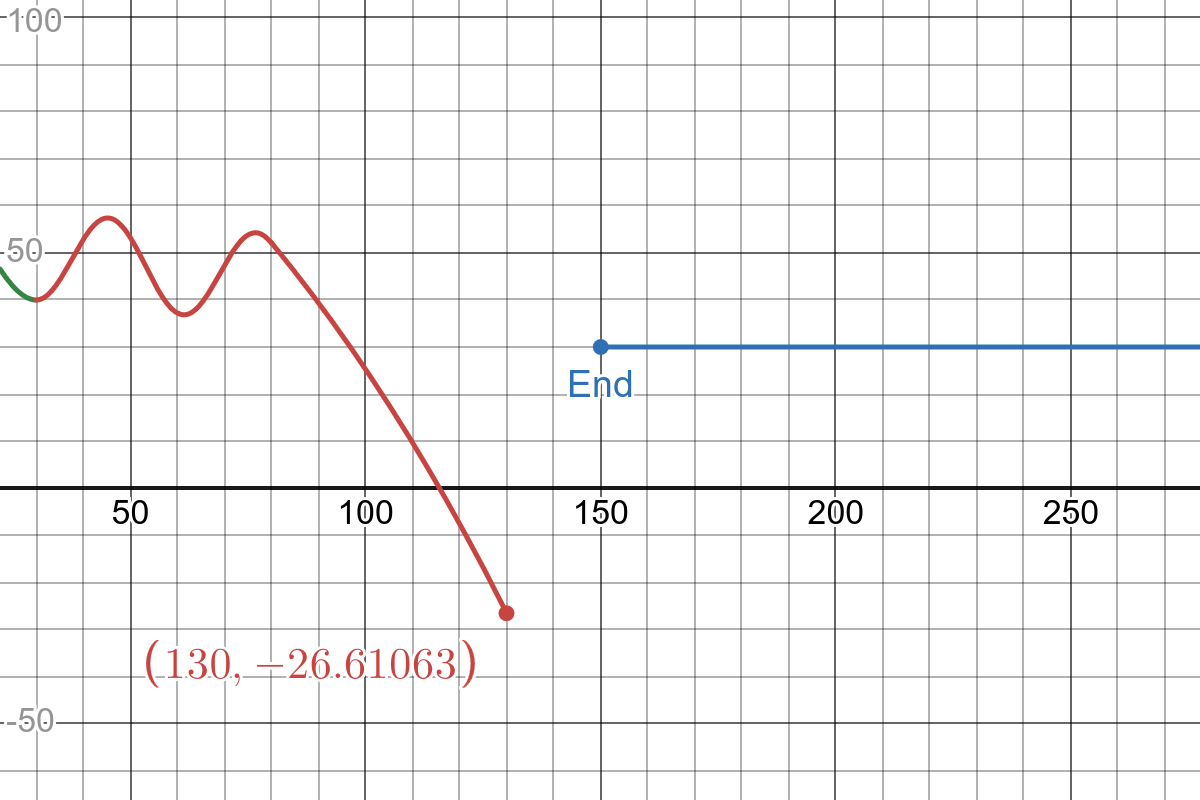
\includegraphics[width=15cm]{PrematureIntersecion.png}
		\caption{Graph of $g(x)$ prematurely intersecting with the $x-\textrm{axis}$}
	\end{figure}
	\item Attempting to insert another condition such as $g(50)=10$ causes the equation to become over constrained, therefore another technique must be used. 
	
	\item By considering $s'(\lambda)=g'(0)$, a suitable $x$ value for the starting point of the function was defined, which did not cause over constraint when later conditions were established. 
	\item This was rearranged to give $a=\frac{s'(\lambda)}{b}$, which can be substituted into $g(\gamma)=-2$, which gave $g'(\gamma)=s'(\lambda)e^{\gamma b}$.
		\item Solving for $b$ gave $b=\frac{1}{\gamma}\ln(\frac{-2}{s'(\lambda)})$, which was then substituted back into $g(x)=ae^{bx}$ to give $g(x)=\frac{s'(\lambda)}{\frac{1}{\gamma}\ln(\frac{-2}{s'(\lambda)})}\cdot e^{\frac{1}{\gamma}\cdot \ln (\frac{-2}{s'(\lambda)})\cdot x}$, where $\gamma$ is the distance that the function takes to reach $g'(x)=-2$, and $\lambda$ is the x value that the function starts at, and joins with the previous function, $s(x)$.
		
		\item $x$ was replaced by $(x-\lambda)$ to horizontally shift, and $s(\lambda)-a$ was inserted at the end to vertically shift so that $g(\lambda)=s(\lambda)$.
		
		\item After inserting the equation into desmos, suitable values for $\lambda$ and $\gamma$ were found. It was required that the equation terminate at $y=10$ so that there would be suitable room for the final function to revert direction and climb. Therefore $g(\lambda + \gamma)=10$, where $\gamma=130-\lambda$ was considered, as this would ensure that $g'(\lambda-\lambda-130)=g'(130)=-2$, while still allowing for $\lambda$ to be altered until a suitable answer was found.
		
		\item It was found that for $g'(130)=-2$ and $g(130)=10$, $\lambda=77.2487110854776$. Therefore $g(x)=\frac{s'(\lambda)}{\frac{1}{\gamma}\ln(\frac{-2}{s'(\lambda)})}\cdot e^{\frac{1}{\gamma}\cdot \ln (\frac{-2}{s'(\lambda)})\cdot (x-\lambda)}+s\left(\lambda\right)-\frac{s'(\lambda)}{\frac{1}{\gamma}}\ln\left(\frac{-2}{s'\left(\lambda\right)}\right)$ where $\lambda=77.2487110854776$, and $\gamma=130-\lambda$.
\end{itemize}




\subsubsection{The Fourth Function}
\begin{itemize}
	\item The final function was decided to be a cubic function, as multiple turning points were required, and the process for defining a cubic with constraints had already been established when creating the first function. 
	
	\item It was required that for the cubic function, say $f_2(x)=a_2x^3+b_2x^2+c_2x+d_2$, $f_2'(130)=g'(130)$, $f_2(130)=g(130), f_2'(150)=0$, and $f_2(150)=30$. 
	
	\item However to simplify calculations, it was considered that $f_2'(0)=g'(130)$, $f_2(0)=g(130), f_2'(20)=0$, and $f_2(20)=30$. Horizontal shift was later accounted for by substituting $x=x-130$
	
	\item Solving simultaneously for these conditions gave values 
	
	$a_{2}=\frac{g'\left(130\right)+40b_{2}}{-1200}$, 
	
	$b_{2}=\frac{3}{400}\cdot\left(30-\frac{g'\left(130\right)\cdot8000}{-1200}-\left(20\cdot g'\left(130\right)\right)-g\left(130\right)\right)$
	
	$c_{2}=g'\left(130\right)$
	
	$d_{2}=g\left(130\right)$

For further working see appendix $\mathbf{A}$
	
\end{itemize}

\subsection{Final Functions and Domains}

$f_1$=


\subsection{Supporting Structures}



\section{Evaluate and Verify}
\subsubsection{Reasonableness}



The assumption that the start and end pieces had a slope of 0 was found to be optimal for smother joining tracks to the  turning points of the inside functions. However, if it was instead assumed that the start and end pieces of track were slanted, with a gradient of, say $-2$, then the roller coaster would be more thrilling, as the passengers would be travelling faster and experience greater forces with the same gradient. 


While simplification of the model to 2D did make the roller coaster less thrilling, as passengers would only experience thrilling movements in 2 dimensions, rather than 3, it greatly simplified calculations as intended


\subsubsection{Strengths}


The function $c(x)$ had the largest changes in gradient, which theoretically contributed the largest thrill to passengers. Additionally, it not only reached the maximum slope naturally throughout its oscillation, but ensured that passengers maintained enough speed to overcome each one of its peaks through its integrated linear function.

While the cubic function was utilised heavily, the requirements for there to be at least two types of functions that were covered in Unit 3 Topic 2 included in the roller coaster and least 3 types of functions overall, were fulfilled.

\subsubsection{Weaknesses}


The organisation and labelling of functions and variables throughout the solution were inconsistent and confusing. A better naming scheme was adopted toward the end of the task, with the last function becoming $f_2$, rather than an arbitrary letter. 

Many variables lacked exact solutions. This resulted in extremely long and complex functions which lacked readability and accuracy. While this was sub optimal, the rounding errors were found to be inconsequential considering the real world scale.


\section{Conclusion}


\section {Bibliography}
\begin{appendices}
	\section{The First Function}
	
	
	\section{The Fourth Function}
	$f_2(0)=g(130)\Rightarrow d=g(130)$
	
	$f_2'(0) = g'(130)\Rightarrow c=g'(130)$
	
	$f'(20)=0\Rightarrow a=1200a+40b+g'(130)$
	
	
\end{appendices}





\end{document}